\documentclass[bachelor,english]{hgbthesis}
% Zulässige Class Options: 
%   Typ der Arbeit: diplom, master (default), bachelor, praktikum 
%   Hauptsprache: german (default), english
%%------------------------------------------------------------

% !TeX spellcheck = en_GB

\graphicspath{{images/}}    % wo liegen die Bilder? 
\bibliography{literatur}  	% Angabe der BibTeX-Datei, % utf8-change

\usepackage{multirow,slashbox,courier,lscape,tablefootnote,hyperref}
\usepackage{longtable}
\usepackage{wrapfig}
\usepackage[toc]{glossaries}

% code listing packages
\usepackage{geometry}
\usepackage{listings}
\usepackage{color}
\usepackage[usenames,dvipsnames,svgnames,table]{xcolor}

\usepackage{pdfpages}
\usepackage{framed}

\usepackage[all]{nowidow}

\usepackage{graphicx}

\usepackage{epigraph}


\setacronymstyle{long-short} % creates example(EX) for the first usage and EX for the following usages of an acronym
\makeglossaries


\loadglsentries{glossary}

% no hyphenation for the following words:
%\hyphenation{example}


%%%----------------------------------------------------------
\begin{document}
%%%----------------------------------------------------------

% use \bigskip for paragraphs that to not belowng to the section anymore. 
% (e.g. conclusions of chapters)
\bigskipamount=30pt

% Einträge für ALLE Arbeiten: --------------------------------
\title{Service Cutter (Working title)}
\author{Michael Gysel \& Lukas K\"{o}lbener}
\studiengang{Computer Science}
\studienort{Rapperswil}
\abgabedatum{2015}{12}{18}	% {YYYY}{MM}{DD}

%%% zusätzlich für eine Bachelorarbeit: ---------------------
%\semester{Spring semester 2015} 
%\gegenstand{Enterprise Application Integration} 
%\betreuer{Olaf Zimmermann} % oder \betreuerin{..}

%\strictlicense  % erzeugt restriktive Lizenzformel

%%%----------------------------------------------------------
\frontmatter
\maketitle
\setcounter{tocdepth}{1}
\tableofcontents
%%%----------------------------------------------------------

\chapter{Abstract}

Decomposing a software system into smaller parts has been an important discipline in our industry for many decades. With the rise of distributed systems, it has become more important to split a system into low coupled and high cohesive parts. Architectural styles like Service Oriented Architecture (SOA) and currently Microservices tackle the many challenges of such systems but remain vague on the art of how to decompose a system into services.

With the help of our industry partner Zühlke, our supervisor Prof. Dr. Olaf Zimmermann, and existing literature, we introduce a structured way to service decomposition by providing a comprehensive coupling criteria catalog.

We embodied these coupling criteria in the Service Cutter, a prototype that extracts coupling information out of well-known concepts like domain models and use cases. Using this information, the Service Cutter’s mission is to produce service cuts to assist an architect’s decomposition decisions. 

A scoring system is defined to automatically interpret coupling data. By employing a weighted, undirected graph and clustering algorithms the Service Cutter produces service cuts that minimize coupling between services while ensuring high cohesion within a service. 

Tests with two sample projects not only met our expectations but produced reasonable service cuts that have not been considered before. 

With a more structured way to service decomposition, the Service Cutter demonstrate that automated decision assistance is a promising way. The thesis lays the foundation for further projects in this area. 
			

%%%----------------------------------------------------------
\mainmatter         % Hauptteil (ab hier arab. Seitenzahlen)
%%%----------------------------------------------------------

% Don't show "Chapter X" titles for every Chapter
\makeatletter
\renewcommand{\@makechapterhead}[1]{%
\vspace*{50 pt}%
{\setlength{\parindent}{0pt} \raggedright \normalfont
\bfseries\Huge\thechapter.\ #1
\par\nobreak\vspace{40 pt}}}
\makeatother


\chapter{Introduction}

This chapter introduces the project's goals, scope and context. The original project definition, signed at the beginning of project, is documented in Appendix \ref{appendix:projectDefinition}.

\section{Hypothesis}

D. L. Parnas published a paper titled \textit{On the Criteria To Be Used in Decomposing Systems into Modules}\cite{parnaDecomposing} in 1972. Since then, decomposition of software systems has become an important area in the field of software engineering. As systems grew more complex, software engineers started to distribute modules over computer networks and hence called them services. Architectural styles like Software Oriented Architecture (SOA) have been introduced to tackle many challenges of such distributed systems.

Nevertheless, even with microservices, the latest incarnation of service orientation, decomposition is more described as an art than a structured discipline. C. Richardson writes in his popular introduction to microservices on \gls{infoq}:

\begin{quote}
	\textit{Deciding how to partition a system into a set of services is very much an art but there are number of strategies that can help. One approach is to partition services by verb or use case.}\cite{richardson2014microservices}
\end{quote}

We consider the described strategies as suitable approaches to service decomposition. However, we assume that service decomposition can be approached in more structured way. This leads us to our first hypothesis:

\begin{quote}
	\textit{The driving forces for service decomposition of a software system can be assembled in a comprehensive criteria catalog.}
\end{quote}

To validate this first hypothesis, we created a comprehensive but not conclusive catalog of coupling criteria as a product of the thesis. Taking this structured approach to service decomposition a step further, we formulated a second hypothesis:

\begin{quote}
	\textit{The data of the criteria catalog can be processed in a software to optimize loose coupling between services and high cohesion within services in a structured and automated way.}
\end{quote}

To validate this second hypothesis, we developed a prototype based on the criteria catalog. This tool, hence called the \enquote{Service Cutter}, analyzes a system's specification and suggests candidate service cuts in order to optimize loose coupling between services and high cohesion within services. A system's specification contains an entity-relation model, use cases, and further artifacts as illustrated in Figure \ref{fig:serviceCutterIO}.

\begin{figure}[H]
	\begin{center}
		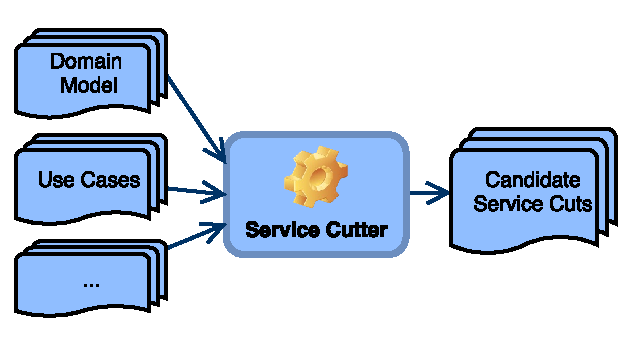
\includegraphics[scale=1.1]{diagrams/systemContextDiagram.pdf}
	\end{center}
	\caption{Input and Output of the Service Cutter}
	\label{fig:serviceCutterIO}
\end{figure}

The Service Cutter's goal is to assist and advise a software architect or developer in his design decisions regarding service decomposition. The architect needs to assess the candidate service cuts and compare them with his expectations. The Service Cutter's mission is accomplished, if the architect's expectations are verified or unexpected but reasonable candidate cuts challenge his preoccupations. 

\section{Project Scope}

This section describes the scope and boundaries of this thesis. 

Throughout the document, a \textit{system} refers to a software application whose architecture needs to be decomposed.

A \textit{service} can be seen as a module providing a remote \gls{API} to communicate with other services. The term is explained in more detail in Chapter \ref{cha:analysis}.

\textit{Service decomposition} refers to splitting a system's functionality and data into services. While we focus on service decomposition, most of the concepts are also true for non-distributed systems where a software internally is decomposed into modules. 

Before a system can be decomposed, its functional and non-functional requirement need be be analyzed and specified in a domain model, use cases, and other artifacts. Based on these specifications the system can be decomposed into services. These are later implemented and connected using intra service communication. Figure \ref{fig:context} illustrates this process.

\begin{figure}[H]
	\begin{center}
		
\includegraphics[scale=1.4]{diagrams/context.pdf}
	\end{center}
	\caption{The thesis in the context of system development}
	\label{fig:context}
\end{figure}

Our thesis focuses solely on service decomposition. Consequently the following areas are not in scope:

\begin{itemize}
	\item Requirements engineering and system specification need to be done before a system can be analyzed with the Service Cutter.
	\item Intra service communication is not in scope of this thesis. S. Newman documents in his book \textit{Building Microservices}\cite{newman2015building} multiple popular ways for intra service communication like \gls{RPC}, RESTful HTTP services or asynchronous event-based collaboration. Decomposition only defines \textit{what} is communicated but now \textit{how}. 
	\item Composing multiple services into workflows or business processes using notations like \gls{BPMN} is not in scope.
	\item Service decomposition tries to minimize coupling between services. Tactics like caches or \gls{CQRS}, which try to lower the consequences of coupling introduced by decomposition, are not analyzed. 
\end{itemize}


\section{Context and Influences}

The ideas and concepts in this thesis are influenced by the work of many others. We reused and embodied existing concepts to our structured way of service decomposition. This section describes the context and influences of the thesis.

\subsection{Service Oriented Architecture}

It was during a course titled \textit{Advanced Distributed Systems Design using SOA \& DDD} by Udi Dahan where our initial idea to assist service decomposition with an automated approach emerged. Dahan is the founder of NServiceBus\cite{nservicebus}, the most popular service bus for \gls{dotnet} and a well known \gls{SOA} and \gls{DDD} expert. The approach to tackle service decomposition from the 4+1 View Model\cite{fourPlusOne} is inspired by him. Approaching decomposition on the basis of data fields, or the later in the document introduced nanoentites, is motivated by his course.

Further \gls{SOA} influences are provided by our supervisor throughout the project and during his course \textit{Application Architecture} at \gls{HSR}.

\subsection{Microservices}

In recent years, microservices substituted \gls{SOA} as the trending architectural style, but can be seen as a new incarnation of the service oriented approach. Valuable concepts like service definitions or decomposition criteria are inspired by leading evangelists in this area such as Martin Fowler, Sam Newman, and Chris Richardson. 

\subsection{Domain-Driven Design}

Nevertheless, decomposition is not solely a problem in distributed systems. Eric Evans introduced in his book \textit{Domain-Driven Design: Tackling Complexity in the Heart of Software}\cite{evans2003domain} a collection of patterns to handle decomposition complexity. Especially the concepts \textit{Aggregate}, \textit{Entity}, \textit{Published Language} and \textit{Bounded Context} are integrated in our approach and serve as input or output of the Service Cutter

\section{Existing Decomposition Solutions}

We were not able to find projects that try to structure and automatically assist service decomposition. Nevertheless, there are several methodologies and decomposition tools tackling some of the relevant challenges. 

\subsection{Software Methodologies}

The already introduced approaches \gls{SOA}, microservices, and \gls{DDD} discuss some decomposition criteria but do not provide a comprehensive criteria catalog. 

Other approaches tackle related problems but are focused on different layers of software development. \gls{OOAD} focuses more on abstractions like classes and object instances. We integrated \gls{OOAD} artifacts like the \gls{ERM} as part of the system description given to the Service Cutter as input. \gls{BPM} lays an abstraction layer above services, focusing on business processes and therefore the usage of services rather than their identification and specification. A detailed analysis on the correlation of \gls{OOAD} and \gls{BPM} with service orientation was published by IBM\cite{zimmermann2004elements}. Service oriented modeling approaches like \gls{SOMA}\cite{arsanjani2004service} target similar questions as this thesis but do not provide detailed description of decomposition approaches. \gls{SOMA} suggests decomposition by use cases which resembles our decomposition criterion \textit{Semantic Proximity} introduced in Chapter \ref{cha:decomposition}.

\subsection{Decomposition Tools}

Kenny Bastani suggests a graph based analysis to decompose monolithic software into microservices\cite{bastani}. In his decomposition approach he focuses on dependencies from user stories to resources. He uses Neo4J GraphGist\cite{graphGist} to visualize the dependencies but does not run any automated analysis on the graph. 

The barrio eclipse plugin\cite{dietrich2008cluster} analyzes dependencies based on Java source code. It suggests a candidate package structure by leveraging the Girvan-Newman clustering algorithm. The tool has been published as part of a students project of the Massey University, New Zealand.

\bigskip

After introducing our hypothesis's and the broader context of service decomposition, the next Chapter analyzes the definition of a service and service decomposition principles in more detail. 

%TODO AppArch 3 Ebenen von Services,  Drei definitionen von SOMA/Services, User / Architect / Developer



\chapter{Analysis}
\label{cha:analysis}



\chapter{Requirements}
\label{cha:requirements}

These chapters describes the (non-)functional requirements of the target solutions and the target users working with the end product.

The requirements in this chapter are not prioritised. As part of the sprint planning meetings, these requirements are transformed and prioritised to user stories and tasks. The description in this chapter is meant to provide a high level overview and establish a common sense between all stakeholders of this project.

\section{Introduction}


\section{Functional Requirements}

The Service Cutter faces the functional requirements presented in the following
section.

%TODO machen wir user stories?

%TODO: each data field needs a master who is the only one doing writes.

%TODO low prio: Add relations between coupling criteria. examples: High volatility and high security is dangerous. Or high criticality and high change management. The Service Cutter could generate warnings if theses things are put together in the same service or either consider theses r


%TODO low prio: Show warnings as part of the output should a predefined service have a significant negative effect!

\subsection{Data Fields and Entities}

A set of data fields can either be defined in the application or imported using a predefined data format. A data field consists of it's name and a combination of connections to other fields, referred to as Coupling Criteria.

The process of putting fields in relation to each other should use as many familiar concepts as possible. The concept of an entity - a set of fields sharing a commdon identity and lifecycle\cite[p.13]{evans2014domain} - is a widely used notion and is therefore used by the architect to model the data and then mapped to the Coupling Criteria \enquote{Shares Lifecycle} and \enquote{Common Identity} by the system.

\subsection{Coupling Criteria}

Almost all data fields are related to other fields. The concept of a Coupling Criterion is used to characterise such connections.

A list of relevant Coupling Criteria was identified in a workshop with Zühlke. The following Criteria are supported by the system:

\begin{itemize}
	\item Shares Lifecycle
	\item Common Identity
	\item Inheritance
	\item Volatility
	\item Security
	\item Resilience
	\item Use Case
\end{itemize}

%TODO liste ergänzen nach workshop!

\subsection{Service Boundaries}

Once the user has added all data fields and coupling criteria he can calculate the suggested service boundaries. An algorithm groups fields in a way that minimizes coupling between the groups while maximizing the cohesion inside a group.

The calculation can be parametrised using weights assigned to coupling criteria. In this way different service boundaries can be calculated for different requirements. For example in an application that processed financial data, security might be more important than Use Cases. In a different context, e.g. for an application that needs to support high volumes of data, volatility and resilience might be a primary focus.

\subsection{Service Coupling}

Some Coupling Criteria will likely span across service boundaries. The architect uses the graphical representation of the Service Cutter to inspect the coupling. Using this information he might change the calculation parameters to achieve a different service cut.

Service Coupling maps to the Published Language as described by Evans \cite[p.375]{evans2003domain}.

% link zu published language von DDD?

% TODO:  Quantification is configurable – but the system provides a good default
\section{Nonfunctional Requirements}
\label{sec:nonfunctionalRequirements}

The following non-functional requirements should be satisfied by the Service Cutter.

\subsection{Usability}
\label{sec:usability}

A software architect should be able to use the software without any training. All controls are clearly named and, where appropriate, documented using an inline user manual including representative samples.

The user gets well introduced to the important concepts of the Service Cutter. These concepts include:

\begin{enumerate}
	\item A Service and service decomposition
	\item A system's model (nanoentities)
	\item Coupling criteria, their meaning and decomposition impact
	\item User representations and their impact on coupling criteria
	\item Characteristics values, coupling criteria priorities and final ratings.
\end{enumerate}

Often used configuration like coupling criteria priorities should be shown directly to the user to encourage its usage. More advanced configuration like the weights of coupling criteria variants should be accessible for the user but do not need to be shown directly in a standard workflow. 

Up to 2000 nanoentities and 200 entities need to be manageable without losing track.

\subsection{Simplicity}

A simple system analysis can be achieved with not more than 5 clicks. All steps are provided with useful defaults that can be changed.

\subsection{Performance}

All regular user interactions should not take more than one second.

Calculations of service cuts should meet the following conditions assuming a data set of 100 entities and 2000 nanoentities.

\begin{itemize}
\item Calculations that are used once per day should take less than 10 minutes.
\item Calculations that are used once per minute should take less than 5 seconds.
\end{itemize}

\subsection{Monitoring, Logging, Deployment, Availability}

The scope of this thesis is to prototypically implement the Service Cutter. Operational aspects only need to be covered on a basic level:

\begin{itemize}
	\item Log files should be written using SLF4J\cite{slf4j}.
	\item Deployment should be provided with Docker\cite{docker} containers.
\end{itemize} 

\subsection{Fault Tolerance}

As the prototype does not need to handle ever possible use case or unexpected input, a common error handling needs to be built into the application and ensures that operations continue even in case of unexpected input or state.

\subsection{Maintainability}

In case of a success the prototype might be the basis for further development or other thesis projects. It should be built in clearly separated modules (or even remote services) to ensure good maintainability. At least the following modules need to be clearly separated:

%TODO thesis plural

\begin{enumerate}
	\item Internal representation of coupling criteria
	\item Data of a users system (nanoentities, use case definition etc.) 
	\item Decomposition algorithm (Solver)
	\item User interface
\end{enumerate}

If one or multiple of the modules are implemented as physical services the remote \gls{API} needs to be implemented as RESTful HTTP interface. 

The application should leverage existing open source frameworks or libraries wherever possible to ensure a minimal maintenance effort.

\subsection{State-of-the-Art Technology}

To support further development of the Service Cutter the prototype needs to be implemented in state-of-the-art technology. Our industry partner Z\"uhlke has suggested the following technology stack:

\begin{enumerate}
	\item Java Spring\cite{spring} as a base framework. 
	\item JHipster\cite{jhipster} with Spring Boot\cite{springboot} for project setup.
	\item AngularJS\cite{angularjs} and Bootstrap\cite{bootstrap} for the user interface.
	\item Docker\cite{docker} for container and deployment configuration and handling. 
\end{enumerate}

\subsection{License}

All involved parties decided to release the Service Cutter under the terms of the Apache 2.0 open source license.

\bigskip

After defining all (non-)functional requirements, the next Chapter outlines design and implementation steps which were taken to satisfy these requirements.


\chapter{Design and Implementation}
\label{cha:implementation}


\section{Design} 


\subsection{Technology}


\subsection{Infrastructure}



\bigskip
After covering the important design and implementation aspects, the next chapter assesses the built solution described in this chapter against the defined requirements.

\chapter{Conclusion}


%%%----------------------------------------------------------
%%%Anhang
\appendix

\chapter{Project Management}
\label{cha:projectmgmt}

This Appendix documents aspects of project management like methodology, roles, environment, quality management, and risk management. The project was time boxed and started on \formatdate{14}{9}{2015} and ended on \formatdate{18}{12}{2015} which implies 14 working weeks. 


%\section{Project Management Methodology}

We chose Scrum as the project management methodology for this bachelor thesis. Scrum specifies an iterative and incremental approach which encourages a high involvement of the customer. This characteristics suit the requirements of a bachelor thesis well,
as it provides only a short project definition at project start and, in our case, requires close collaboration with our advisor and industry partner.

%\clearpage
\section{Project Roles}

Scrum defines three project roles — the product owner, the scrum master and the development
team. As this bachelor thesis is an academical project, the scrum roles could
not be mapped one to one. This Section introduces the involved persons and their roles
in the project.

\subsection{HSR Supervisor}

\begin{minipage}[t]{0.25\textwidth}
	\vspace{0pt}
	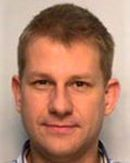
\includegraphics[width=0.8\textwidth]{olz.jpg}
\end{minipage}
\begin{minipage}[t]{0.8\textwidth}
	\vspace{10pt}
	Prof. Dr. Olaf Zimmermann is the \gls{HSR} supervisor of this thesis and incorporates both, the role of the product owner and scrum master. \textit{Product} in this context refers to the thesis itself as well as the functional product. He ensures that all requirements by HSR for a bachelor thesis are met and decides in last instance about the scope of the thesis. 
	As supervisor and coach of the development team, Mr. Zimmermann also performs part of the scrum master role as he coaches the development team.
\end{minipage}


\subsection{Industry Partner}

Our industry partner Zühlke Engineering, represented by W. Giersche, ensured the functional relevancy of this thesis. Mr. Giersche contributed valuable experience from many software engineering projects. He represented part of the product owner role as he played an important role in the functional prioritization to maximize the business value. Being an experienced software architect, he also contributed to the coupling criteria catalog by conducting workshops.


\subsection{Project Team}

Michael Gysel and Lukas Kölbener formed the development team. They worked as an interdisciplinary team in which both were responsible for each part of the project. Both being Certified ScrumMasters\textregistered\cite{scrummaster}, they incorporated part of the scrum master role as they helped maintaining the product backlog and organized everything for correct sprint operation.

\begin{minipage}[t]{0.25\textwidth}
	\vspace{0pt}
	
\includegraphics[width=0.8\textwidth]{lukas.jpg}
\end{minipage}
\begin{minipage}[t]{0.8\textwidth}
	\vspace{20pt}
	Lukas Kölbener is an information technology student at \gls{HSR} in his 9\textsuperscript{th} semester. He works part time as Java developer for Super Computing Systems AG in Zurich, building ticket vending machines for the public transport industry.
	\newline
\end{minipage}

\begin{minipage}[t]{0.25\textwidth}
	\vspace{0pt}
	
\includegraphics[width=0.8\textwidth]{michi.jpg}
\end{minipage}
\begin{minipage}[t]{0.8\textwidth}
	\vspace{20pt}
	Michael Gysel is an information technology student at \gls{HSR} in his 9\textsuperscript{th} semester. He works part time as Java Developer for FIS, a global provider for banking and payments technologies.
	\newline
\end{minipage}

%\section{Development Environment}

Figure \ref{fig:devenvironment} outlines all components of the development environment. The Service Cutter is developed with Java 8 using Eclipse Mars~\cite{eclipsemars}. \gls{HSR} has provided a \gls{VM} on which the \gls{docker} images are running. On the same server a \gls{CI} Jenkins server pulls for changes from the Git repositories on GitHub to build and test the different projects. The Docker images are built using a Maven plugin on Jenkins and then pushed into the local Docker repository. Table \ref{tab:vm} indicates the software installed by us on the server.


\begin{table}[H]
\begin{center}
\begin{tabular}
{|p{100pt} p{80pt}|}
\hline \textbf{Software} & \textbf{Version} \\ 
\hline Java & 1.8.0\_60 \\ 
\hline Jenkins & 1.629 \\ 
\hline Docker & 1.8.2 \\ 
\hline Docker Compose & 1.4.1 \\
\hline Apache Maven & 3.0.5 \\
\hline Node.js & 0.10.25 \\
\hline NPM & 1.3.10 \\
\hline 
\end{tabular} 
\caption{Installed software on sinv-56064.edu.hsr.ch (152.96.56.64)}
\label{tab:vm}
\end{center}
\end{table}

\begin{figure}[H]
	\centering{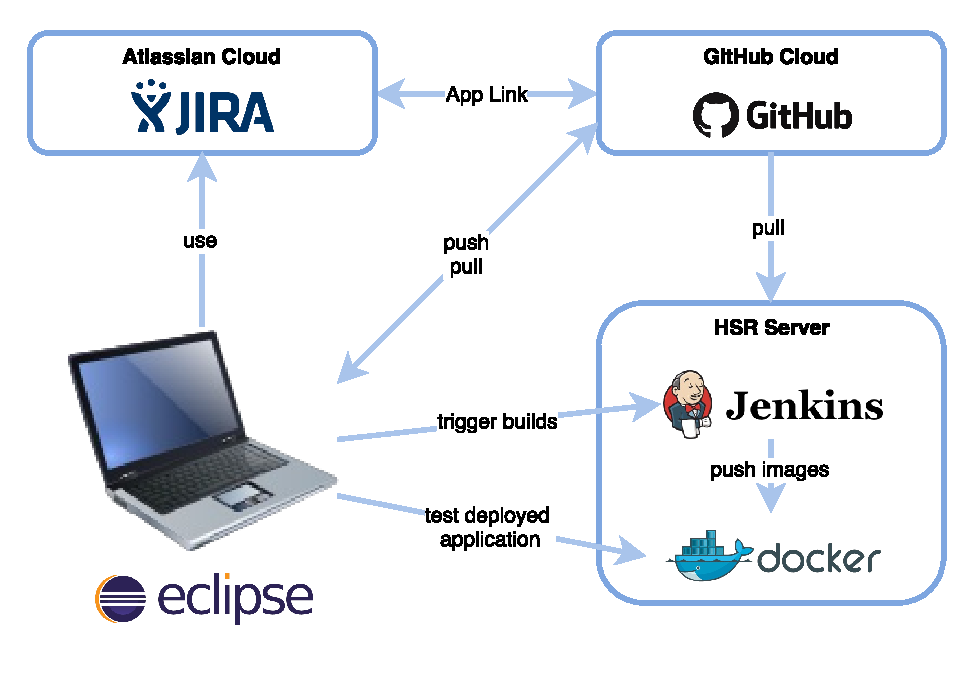
\includegraphics[scale=0.7]{diagrams/DevelopmentEnvironment.pdf}}
	\caption{Development Environment}
	\label{fig:devenvironment}
\end{figure}

%\input{projectmgmt/qualitymgmt}
%\section{Sprint Plan}
\label{sec:projplan}

The project is organized in 4 regular sprints with each two weeks length. 

\begin{itemize}
\item 1st Sprint: \formatdate{14}{09}{2015} - \formatdate{25}{09}{2015}
\subitem Refinement of thesis concept
\subitem Implementation of prototype
\item 2nd Sprint: \formatdate{12}{10}{2015} - \formatdate{23}{10}{2015}
\subitem Development of algorithm
\subitem Development of Coupling Criteria catalog
\item 3rd Sprint: \formatdate{09}{11}{2015} - \formatdate{20}{11}{2015}
\subitem Finish functional requirements
\subitem Test significantly large project
\item 4th Sprint: \formatdate{30}{11}{2015} - \formatdate{11}{12}{2015}
\subitem Refine scoring system, fine tune sample models
\item 5th Sprint: \formatdate{14}{12}{2015} - \formatdate{18}{12}{2015} (one week)
\end{itemize}

The 5th sprint will solely be used to finish the documentation.

%TODO müssen wir beschreiben, was wir zwischen den sprints machen?

\section{Hours Worked}

We invested a total of 757 hours on this project. Michael Gysel worked 365 hours and Lukas Kölbener spent 392 hours on this thesis. Figure \ref{fig:hoursworked} breaks these numbers down into individual categories. We tracked them using epics which is a common technique in agile projects.

\begin{figure}[H]
	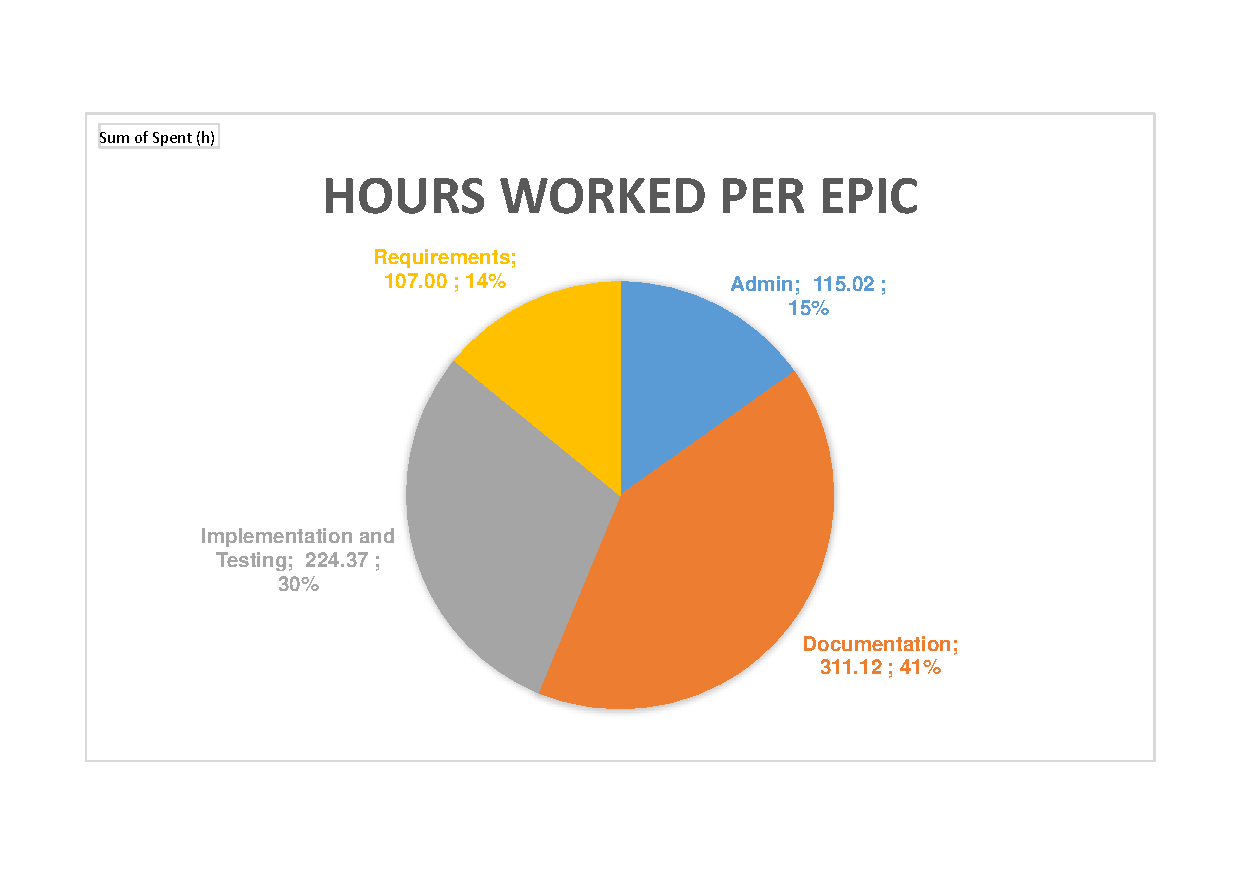
\includegraphics[scale=0.7]{diagrams/hoursperepic.pdf}
	\caption{Development Environment}
	\label{fig:hoursworked}
\end{figure}
%\include{projectmgmt/risk_management}

%\include{anhang_a}	% 
%\include{anhang_b} % 
%\include{anhang_c} % 
%\include{anhang_d} % 
%\include{anhang_e} % 

%\renewcommand{\glossarypreamble}{Descriptions of Glossary items have mainly been taken from Wikipedia.org.\newline\newline}

\printglossaries


%%%----------------------------------------------------------
\MakeBibliography
%%%----------------------------------------------------------


\end{document}
